\section{Design}

\begin{figure}[ht] 
\begin{center}
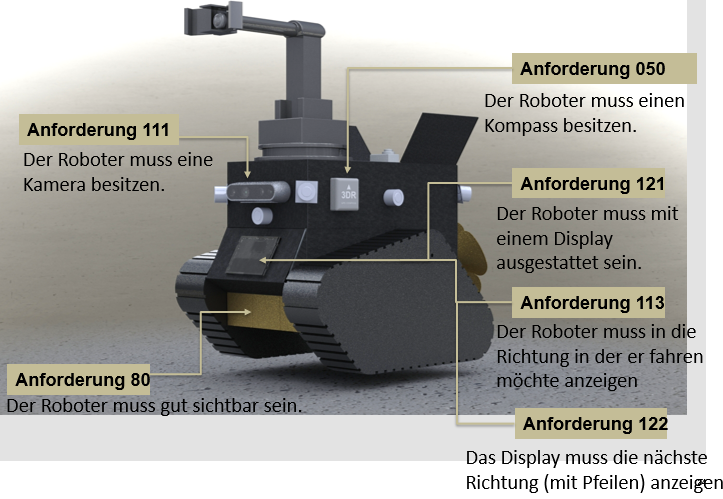
\includegraphics[width = 0.7\linewidth] {Vorne.png}
\caption{Rescue Robot Vorne}
\end{center}
\end{figure}

Auf dem Fig.4 ist unser fertiges Rendering vom Rescue Robot zu sehen.
Jedes einzelne Bauteil ist mit den zu erfüllenden Anforderungen verbunden. Diese Verbindung wird mit einem Pfeil dargestellt.

\subsection{Multifunktionskamera}
(Anforderung: 111)

Hier zu sehen ist unsere Multifunktionskamera. Diese besteht aus einer Infrarotkamera, einer Thermalkamera, einer Nachtsichtkamera und einer Digitalkamera.
Sie wird genutzt, um Objekte und Personen während der Fahrt in der Ferne zu erkennen.

\subsection{Led Panel}
(Anforderung: 80)

Die Anforderung 80 zeigt ein dreiteiliges LED Panel, welches für die Beleuchtung genutzt wird.
Zudem hilft das Licht des LED Panel dem Bediener und macht den Rescue Robot gut sichtbar für die Umgebung.

\subsection{GPS/Kompass}
(Anforderung: 50)

An der Seite des Roboters wurde 
der Multifunktions GPS/Kompass angebracht, 
um die richtige Richtung 
und den aktuellen Standort zu ermitteln.

\subsection{Display}
(Anforderung: 113/121/122)

Vorne am Robot und gut sichtbar, wurde das Display angebracht.
Hier werden Nachrichten für die Umgebung dargestellt. Wie z.B das Blinken mit einem Pfeil in die Richtung, wohin er fährt. Zusätzlich kann auch über das Display, mit dem Patienten, kommuniziert werden.
 
\subsection{Kran mit Mutlimedia-Globe}
(Anforderung: 70/113)

Oben, auf dem Robot, ist der bewegliche Kran befestigt.
Die Hauptaufgabe des Krans ist es, den Patienten sicher zu bergen und in den Rescue Robot zu legen.
Der Kran wird auch dafür verwendet um kleinere Gegenstände, die im Weg liegen, zu entfernen.
Dies geschieht über die extra angefertigte Kralle, die auch für einen sicheren Transport des Patienten sorgt.
Der Kran ist ausfahrbar und kippbar um die Person auch aus schweren Situationen zu retten.
Zusätzliche ist ein Multimedia-Globe befestigt. Dieser beinhaltet eine Kamera, einen Lautsprecher und ein Mikrofon, um mit der zu rettenden Person zu kommunizieren.


\begin{figure}[ht] 
\begin{center}
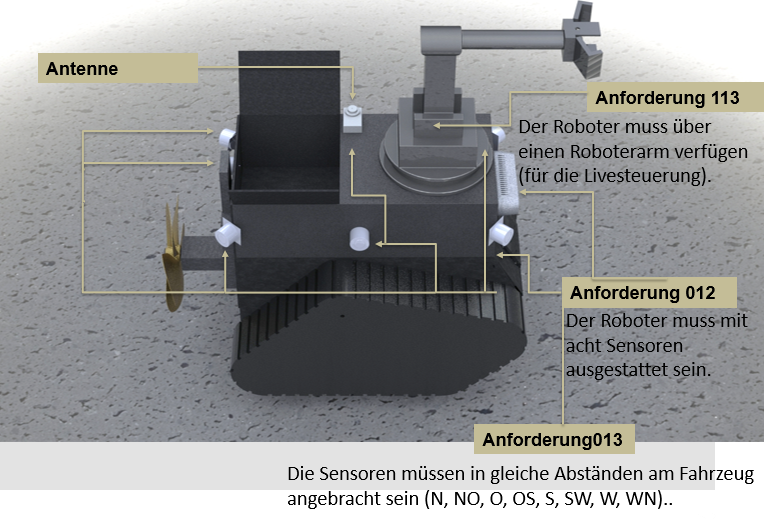
\includegraphics[width = 0.7\linewidth] {Oben.png}
\caption{Rescue Robot Oben}
\end{center}
\end{figure}

\subsection{Abstandssensoren}
(Anforderung: 012/013)

In allen Himmelsrichtungen sind Abstandssensoren an den Robot angebracht.
Diese sorgen dafür, dass unser Rescue Robot die Umgebung erfassen kann und Hindernisse frühzeitig erkennt.

\subsection{Antenne}
Oben auf dem Robot wurde eine Antenne befestigt um Signale zu empfangen.

\begin{figure}[ht] 
\begin{center}
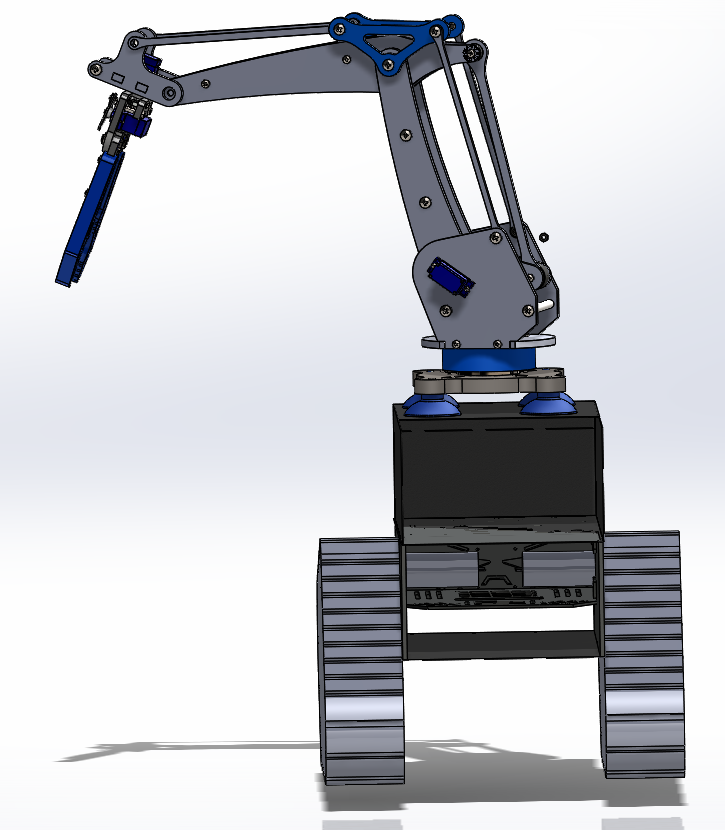
\includegraphics[width = 0.7\linewidth] {Hinten.png}
\caption{Rescue Robot Hinten}
\end{center}
\end{figure}
\newpage

\subsection{Wasserantrieb}
(Anforderung: 031/043)

Hinten am Rescue Robot ist eine Schiene befestigt, um den daran befestigten Propeller hoch und runter fahren zu können.
Der Propeller wird für den Wasserantrieb verwendet.


\subsection{Ketten}
(Anforderung: 044)

Zu sehen sind große stabile Ketten um auf dem Land über mehrere Hindernisse zu fahren.

\subsection{Doppeltür}
Die automatisch öffnenden/schließenden Türen oben am Robot sind dafür da, dass die Person sicher zurückgebracht werden kann, ohne das z.B Trümmer oder gar Feuer in das Fahrzeug gelangen kann.

\begin{figure}[ht] 
\begin{center}
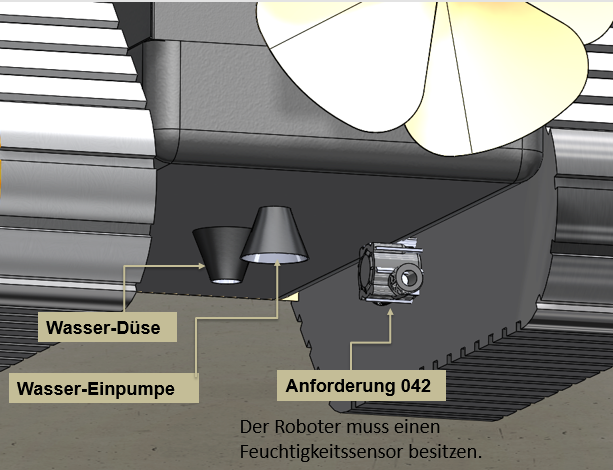
\includegraphics[width = 0.7\linewidth] {Unten.png}
\caption{Rescue Robot Unten}
\end{center}
\end{figure}
\newpage


\subsection{Wasser-Düse}
Die unten angebrachte Wasserdüse wird genutzt, um dem Rescue Robot im Wasser Auftrieb zu geben, da er durch sein Gewicht nicht schwimmen kann.

\subsection{Wasser-Einpumpen}
Bei der Wasser-Einpumpe wird das Wasser 

für die Wasserdüse eingepumpt.

\subsection{Feuchtigkeitssensor}
(Anforderung: 042)

Der Feuchtigkeitssensor stellt fest, ob der Robot im Wasser ist und auf seinen Wasserantrieb wechseln muss.


\begin{figure}[ht] 
\begin{center}
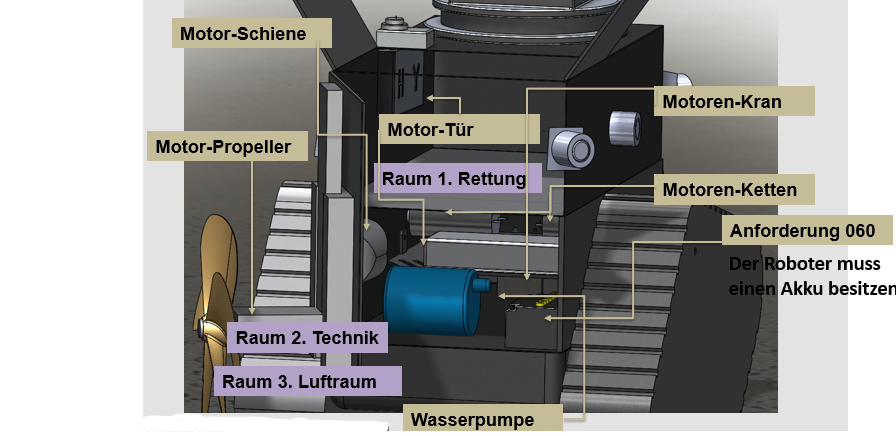
\includegraphics[width = 1 \linewidth] {HintenOpen.png}
\caption{Rescue Robot Offen}
\end{center}
\end{figure}

\subsection{Raum 1}
Im vorderen Raum 1 wird die Person gesichert.
Im hinteren Raum 1 sind die Motoren für das öffnen und schließen der Tür angebracht.

\subsection{Raum 2}
Im Raum 2 sind die meisten Motoren untergebracht, wie die Motoren für die Ketten, den Kran und die Schiene.
Zusätzlich ist dort eine Wasserpumpe und ein Akku untergebracht.
Der Motor für den drehenden Propeller ist in der Schiene an der Tür integriert. 

\subsection{Raum 3}
Der Raum 3 ist für den Auftrieb des Robot gedacht. 
Dieser ist mit Luft gefüllt und sorgt für einen sicheren Auftrieb.







